\documentclass[oneside, 11pt]{article}

\usepackage[T1]{fontenc}
\usepackage[utf8]{inputenc}
\usepackage[dutch]{babel}

\usepackage{fouriernc}
\usepackage[detect-all, load-configurations=binary,
            separate-uncertainty=true, per-mode=symbol,
            retain-explicit-plus, range-phrase={ tot }]{siunitx}

\usepackage{setspace}
\setstretch{1.2}

\setlength{\parskip}{\smallskipamount}
\setlength{\parindent}{0pt}

\usepackage{geometry}
\geometry{marginparwidth=0.5cm, verbose, a4paper, tmargin=3cm, bmargin=3cm, lmargin=2cm, rmargin=2cm}

\usepackage{float}

\usepackage[fleqn]{amsmath}
\numberwithin{equation}{section}
\numberwithin{figure}{section}

\usepackage{graphicx}
\graphicspath{{Figures/}}
\usepackage{subfig}

\usepackage{tikz}
\usetikzlibrary{plotmarks}

\usepackage{fancyhdr}
\pagestyle{fancy}
\fancyhf{}
\rhead{\thepage}
\renewcommand{\footrulewidth}{0pt}
\renewcommand{\headrulewidth}{0pt}

\usepackage{relsize}
\usepackage{xspace}
\usepackage{url}

\newcommand{\figref}[1]{Figuur~\ref{#1}}

\newcommand{\hisparc}{\textsmaller{HiSPARC}\xspace}
\newcommand{\kascade}{\textsmaller{KASCADE}\xspace}
\newcommand{\sapphire}{\textsmaller{SAPPHiRE}\xspace}
\newcommand{\jsparc}{\textsmaller{jSparc}\xspace}
\newcommand{\hdf}{\textsmaller{HDF5}\xspace}
\newcommand{\aires}{\textsmaller{AIRES}\xspace}
\newcommand{\csv}{\textsmaller{CSV}\xspace}
\newcommand{\python}{\textsmaller{PYTHON}\xspace}
\newcommand{\corsika}{\textsmaller{CORSIKA}\xspace}
\newcommand{\labview}{\textsmaller{LabVIEW}\xspace}
\newcommand{\daq}{\textsmaller{DAQ}\xspace}
\newcommand{\adc}{\textsmaller{ADC}\xspace}
\newcommand{\adcs}{\textsmaller{ADC}s\xspace}
\newcommand{\Adcs}{A\textsmaller{DC}s\xspace}
\newcommand{\hi}{\textsc{h i}\xspace}
\newcommand{\hii}{\textsc{h ii}\xspace}
\newcommand{\mip}{\textsmaller{MIP}\xspace}
\newcommand{\hisparcii}{\textsmaller{HiSPARC II}\xspace}
\newcommand{\hisparciii}{\textsmaller{HiSPARC III}\xspace}
\newcommand{\pmt}{\textsmaller{PMT}\xspace}
\newcommand{\pmts}{\textsmaller{PMT}s\xspace}

\DeclareSIUnit{\electronvolt}{\ensuremath{\mathrm{e\!\!\:V}}}

\DeclareSIUnit{\unitsigma}{\ensuremath{\sigma}}
\DeclareSIUnit{\mip}{\textsmaller{MIP}}
\DeclareSIUnit{\adc}{\textsmaller{ADC}}

\DeclareSIUnit{\gauss}{G}
\DeclareSIUnit{\parsec}{pc}
\DeclareSIUnit{\year}{yr}



\title{Data retrieval}
\author{A.P.L.S. de Laat} 
\docanalyse{2}{DR}
\version{1.0}

\begin{document}

\maketitle

\section{Toegang tot \hisparc gegevens}

De data opslag van \hisparc meetgegevens gebeurt op het Nikhef en
bestaat uit een paar databases. Als eerst is er de ruwe dataopslag.
Daarin worden metingen opgeslagen zodra ze naar het Nikhef worden
gestuurd. Daarnaast is er nog een afgeleide database. In de afgeleide
database zijn al een aantal analyses op de meetgegevens uitgevoerd. Met
name de aankomst tijden van de shower in verschillende detectoren en het
aantal deeltjes in een detector.

Toegang tot \hisparc meetgegevens is vrij voor iedereen. Het downloaden
van de ruwe data is niet heel eenvoudig, bovendien raden we dat ook niet
meer aan nu de afgeleide database beschikbaar is. Data uit de afgeleide
database wordt als csv-bestand (tab gescheiden kolommen) aangeboden voor
download via deze website: \url{http://data.hisparc.nl/data/download}.

Zodra data gedownload is kan deze bijvoorbeeld in Excel geïmporteerd
worden om grafieken te maken en analyses uit te voeren. Omdat Excel niet
altijd even eenvoudig werkt hebben we zelf een programma gemaakt dat in
webbrowsers werkt. Het download data en kan daar direct grafieken mee
maken.


\section{\jsparc bibliotheek}

\jsparc is de JavaScript bibliotheek die het makkelijker maakt om met
\hisparc data te werken. Zo biedt de bibliotheek een eenvoudige functie
om gegevens op te halen van de \hisparc server en deze gelijk om te
zetten tot een formaat dat begrijpelijk is voor JavaScript. De broncode
is hier te vinden: \url{https://www.github.com/hisparc/jsparc/}.


\section{Data retrieval}

Dit is een beschrijving van de pagina te bereiken via
\url{http://data.hisparc.nl/media/jsparc/data_retrieval.html}. Hiermee
kan data opgehaald en bestudeerd worden. Aan het \hisparc logo (rechts
boven) is te herkennen of de pagina data van de \hisparc server aan het
ophalen is, dan is het logo namelijk geanimeerd. Als eerst haalt de
pagina een up-to-date lijst van \hisparc stations op, dit gaat zo snel
dat het logo maar heel kort geanimeerd is. Onder het logo is een knop om bij 
de documentatie van de pagina te komen: \url{http://doc.hisparc.nl/jsparc/}.


\subsection{Downloaden van data}

Het Download data formulier, zie \figref{fig:get_data}, staat toe
een \hisparc station, een start- en einddatum, en het data type te
selecteren. Door te drukken op \emph{Get Data!} wordt de data dan
gedownload. Zodra de nieuwe data is geladen, verschijnt er een nieuwe
sectie op de pagina die een overzicht weergeeft van alle datasets die
geladen zijn, zie \figref{fig:data_overview}. Het is mogelijk meerdere
datasets te laden door het Download data formulier opnieuw te gebruiken
met andere instellingen. Met het rechter formulier; \emph{Load local
file} kan eigen of eerder gedownloade .csv bestanden (tab
gescheiden) inladen. Deze verschijnen dan ook in het overzicht.

\begin{figure}
    \centering
    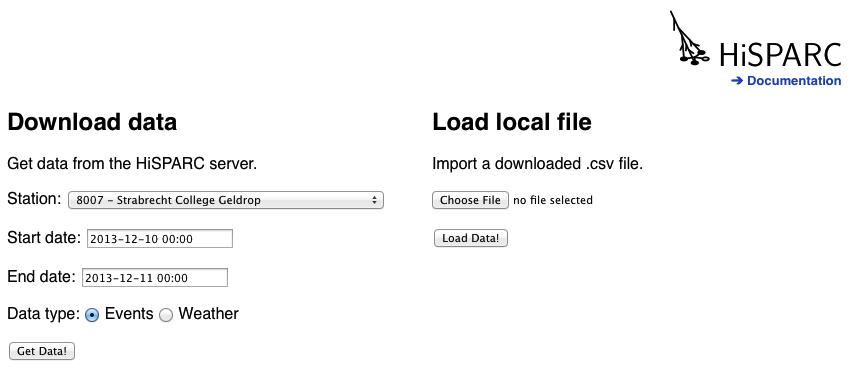
\includegraphics[scale=0.4]{get_data}
    \caption{Gedeelte van de website waar data mee gedownload of
             ingeladen kan worden.}
    \label{fig:get_data}
\end{figure}

\begin{figure}
    \centering
    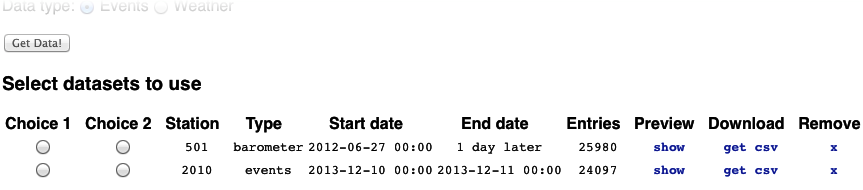
\includegraphics[scale=0.4]{data_overview}
    \caption{Overzicht van de ingeladen datasets.}
    \label{fig:data_overview}
\end{figure}

Met de geladen datasets kunnen verschillende acties uitgevoerd worden.
Door in de \emph{Choice} kolommen een dataset te kiezen verschijnen de
plot opties en een lijst van de variabelen in die dataset. In sectie
\ref{subsec:plotting} is uitgelegd wat alle opties betekenen. Daarnaast
kan er gekozen worden om de waarden in de dataset te bekijken door op
\emph{show} te klikken in de \emph{Preview} kolom. Met de \emph{get csv}
knop wordt het .csv bestand gedownload. Met de \emph{x} in de
\emph{Remove} kolom kan de dataset uit het geheugen van de browser
gewist worden.


\subsection{Grafieken maken}\label{subsec:plotting}

Zodra een dataset gekozen is kunnen er plots (grafieken) mee gemaakt
worden. Er zijn 3 opties voor soorten grafieken. Bij het type
\emph{scatter} worden er twee variabelen voor iedere meting tegen elkaar
uitgezet, een op de x-as en de ander op de y-as. Bij het type
\emph{histogram} kan maar één variabele gekozen worden (x-as). Bij een
histogram wordt het hele bereik tussen de minimale en maximale waarde
van die variabele opgedeeld in een aantal (normaal 100) evengrote delen.
Dan wordt voor elke individuele waarde gekeken in welk bereik die past,
het aantal waarden in een bereik komt dan op de y-as te staan. Als
laatste is er nog de \emph{time series}. Hierbij is de x-as de tijd (en
datum) en kan een variabele voor de y-as gekozen worden.

Als de keuzes gemaakt zijn kan de plot gemaakt worden door op
\emph{Create Plot} te drukken, zie \figref{fig:plot}. Als de opties
aangepast worden kan een nieuwe plot gemaakt worden door weer op die
knop te drukken.

In sommige gevallen zal je meerdere kleuren zien de grafiek dat komt
doordat bepaalde variabelen door meerdere sensoren of detectoren gemeten
worden. Met kleur codes wordt dan aangeven om welke detector het gaat.
In het geval van \hisparc metingen is zwart detector 1, rood detector 2,
groen detector 3 en blauw detector 4. Bij weermetingen met meerdere
sensoren is zwart de binnen sensor en rood de buiten sensor.

\begin{figure}
    \centering
    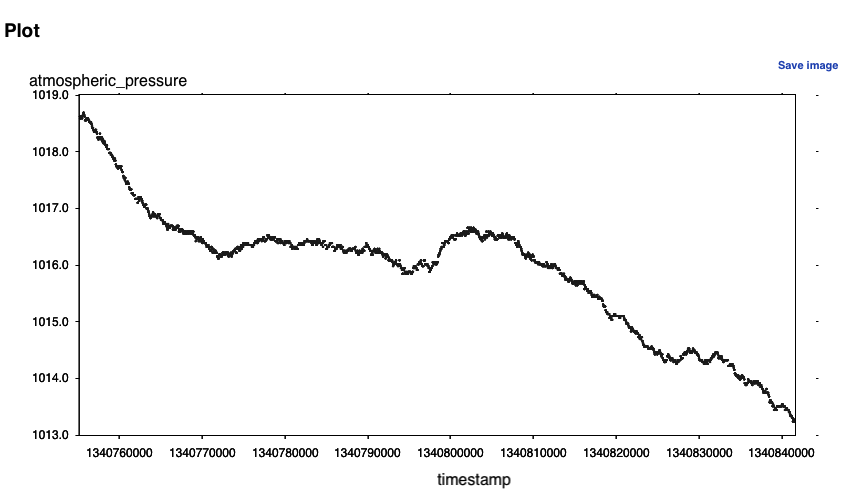
\includegraphics[scale=0.4]{plot}
    \caption{Voorbeeld van een plot. Hier is de luchtdruk op de y-as
             uitgezet tegen de tijdstempel op de x-as.}
    \label{fig:plot}
\end{figure}


\subsection{Interpolatie}

Als meerdere datasets zijn opgehaald met overlappende tijdperiodes is
het mogelijk om deze tegen elkaar te plotten. Kies hiervoor een dataset
in kolom \emph{Choice 1} en de ander in \emph{Choice 2}. De variabelen
verschijnen dan naast elkaar, zie \figref{fig:plot_options_1}. Nu kan uit
beide een keuze gemaakt kan worden voor de x- en y-assen. De
interpolatie vindt plaats op basis van de tijdstempels van de gegevens.

\begin{figure}
    \centering
    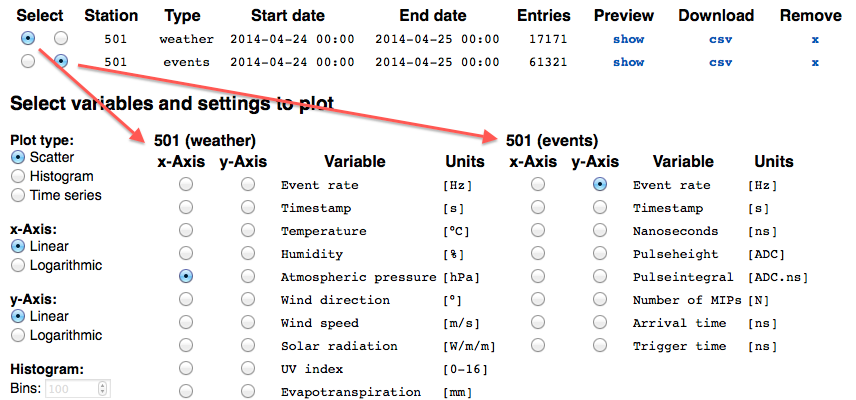
\includegraphics[scale=0.4]{plot_options_1}
    \caption{Meerdere datasets kiezen uit het overzicht.}
    \label{fig:plot_options_1}
\end{figure}


\subsection{Gegevens inkijken}\label{subsec:gegevens}

Door op de knop \emph{show} te drukken in het overzicht van de datasets
verschijnt een tabel met op elke rij in kolommen verdeelt de waardes van
een meting, zie \figref{fig:data_preview} voor een voorbeeld. Niet alle
rijen worden direct getoond, het kost de browser namelijk te veel tijd
om duizenden regels te tonen, dus eerst worden er zo'n 30 getoond, door
op de middelste regel te klikken ('click to show more') kan er meer
ingekeken worden. Hier is ook duidelijk te zien dat sommige kolommen
meerdere waarden hebben, omdat die waarden door meerdere sensoren of detectoren
gemeten zijn. Voor deze waarden gelden dezelfde kleur aanduidingen als bij 
de grafieken.

\begin{figure}
    \centering
    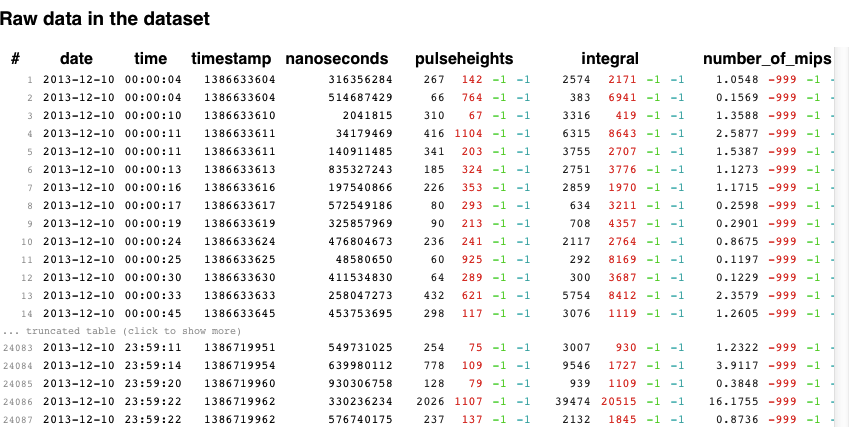
\includegraphics[scale=0.4]{data_preview}
    \caption{Overzicht van de meetwaarden in een dataset.}
    \label{fig:data_preview}
\end{figure}


\subsection{Traces bekijken}

Van iedere detectie van een air shower zijn de signalen uit de \pmts te
bekijken. Gebruik eerst de knop om de gegevens in te kijken zoals
beschreven in sectie \ref{subsec:gegevens}. Ga dan naar de kolom met de
kop \emph{Traces}, druk daar op de \emph{show} knop van een event. Dan
zullen de \pmt signalen worden opgehaald van de server en worden getoond
als grafiek, zie \figref{fig:event_traces}.

\begin{figure}
    \centering
    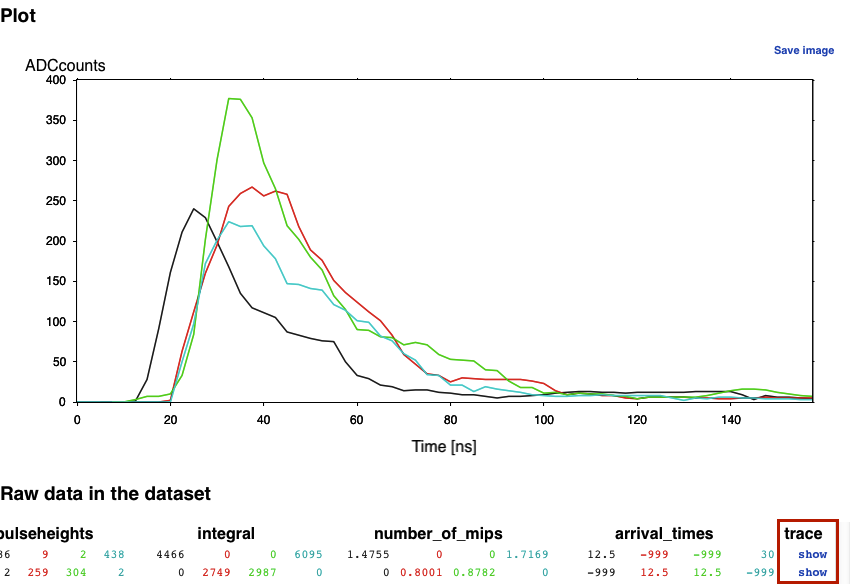
\includegraphics[scale=0.4]{event_traces}
    \caption{De traces van een meting. De met rood gearceerde kolom
             bevat de knoppen om de traces voor een event op te halen.}
    \label{fig:event_traces}
\end{figure}


\subsection{Fitten van data}

Met de dataretrieval tool kan van opgevraagde datasets ook een functie-fit geplot 
worden. Als variabelen geselecteerd zijn, klik dan op het formulier \emph{Fit:} 
om een fit optie te kiezen. Als fit-keuze verschijnen dan \emph{No fit; Linear;
Exponential; Logarithmic; Power; Polynomial.} Bij de optie \emph{Polynomial} 
kun je de macht van de polynoom reeks aangeven bij \emph{Degree}.
Door nu op op \emph{Create Plot} te klikken, krijg je een plot van de variabelen
en een fit van de datapunten te zien. Onder het plotje verschijnt de vergelijking 
van de fit curve. Zie \figref{fig:plot_options_fit}.

\begin{figure}
    \centering
    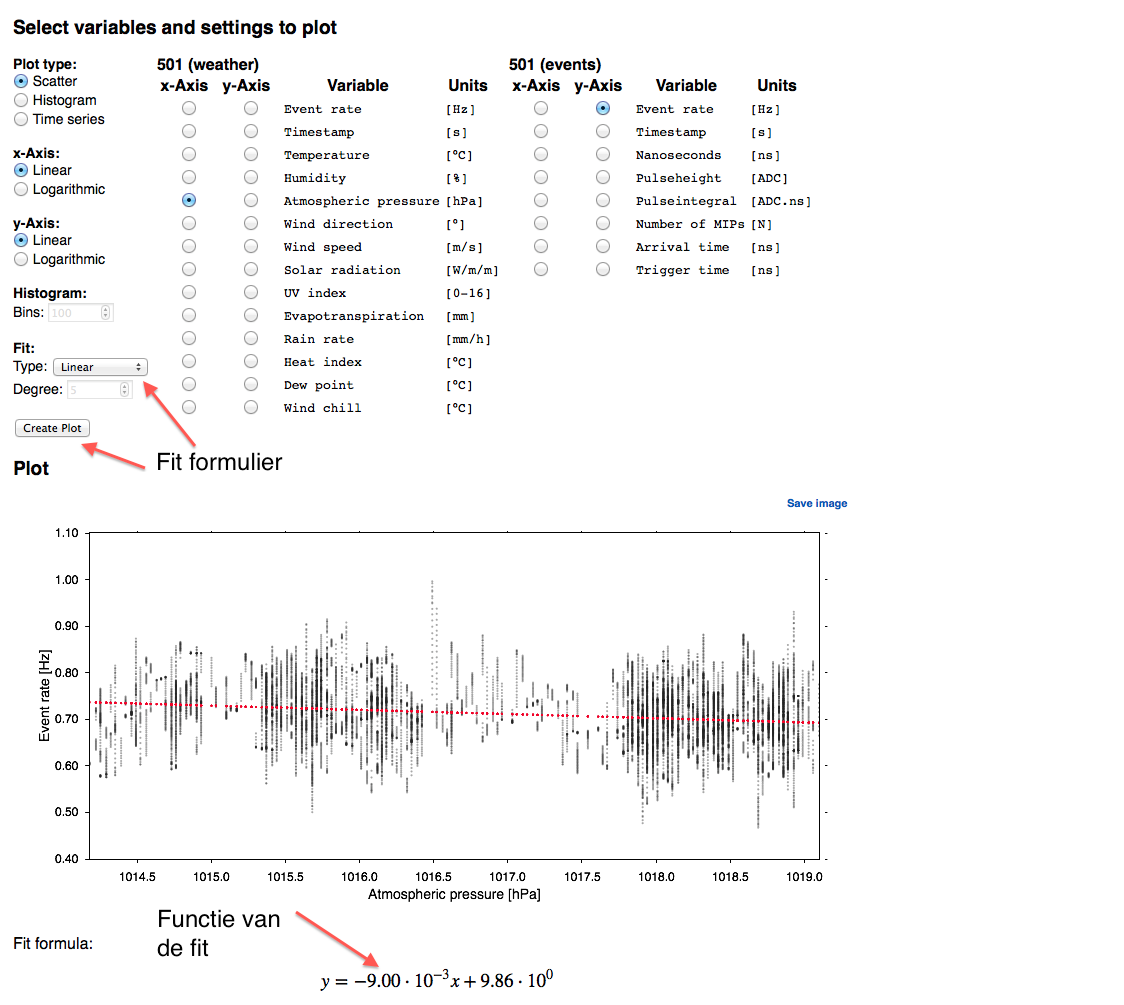
\includegraphics[scale=0.4]{plot_options_fit}
    \caption{Instellen van een fit van twee variabelen. Hier bijvoorbeeld 
    event rate tegen luchtdruk}
    \label{fig:plot_options_fit}
\end{figure}

%\begin{thebibliography}{9}
%\end{thebibliography}

\end{document}
